% Results
\section{Results and Evaluation}
Upon training the model using, we observed promising results in terms of accuracy. Tables and graphs were constructed of our validation and testing data with the help of MATLAB and Excel features to analyze the data and assess the accuracy of our trained model.

\subsection{Validation Results}
The success percentage of the diet recommendation system for the validation data was found to be very promising, yielding high rates of correct recommendations for each specific food/nutrient group. \textbf{Table II} summarizes the overall validation results, which presents the performance of dietary recommendations across different diet types (DT). Out of 345 total recommendations for each diet type, the model correctly predicted the majority, with a few incorrect predictions. The overall success rate, representing the accuracy of the recommendations, is remarkably high at 97.29\%.

\begin{table}[H]
    \centering
    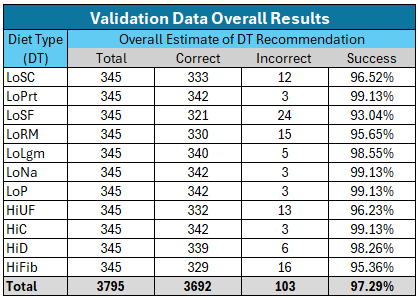
\includegraphics[width=\linewidth]{Figures/vdor.png}
    \caption{Results of the overall validation data.}
\end{table}

\textbf{Table III} shows the total number of instances where a diet type (DT) was recommended, along with the number of correct and incorrect predictions. Among the 1,674 recommendations, the model correctly identified 1,654 instances, achieving an overall accuracy of 98.81\%.
For instance, the diet type Low Simple Carbohydrates (LoSC) was recommended 278 times, with the model correctly predicting 277 of those recommendations, resulting in a success rate of 99.64\%. Similarly, the model achieved perfect accuracy of nearly 100\% for diet types such as Low Protein (LoPrt), Low Red Meat (LoRM), Low Sodium (LoNa), and Low Phosphorus (LoP). This high level of accuracy across various diet types demonstrates the model's effectiveness in making precise dietary recommendations when specific diet types are required.

\begin{table}[H]
    \centering
    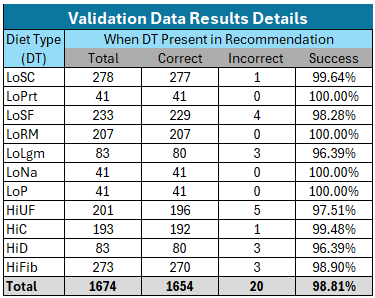
\includegraphics[width=\linewidth]{Figures/vdrdp.png}
    \caption{Results of the validation data when diet type was present in recommendation.}
\end{table}

\textbf{Table IV} shows the total number of instances where a diet type (DT) was not recommended. Among the 2121 recommendations, the model correctly identified 2038 instances, achieving an overall accuracy of 96.09\%.The incorrect predictions happen mostly when a diet type is not recommended to the patient (False Positive). LoSC, LoSF, LoRM and HiFib diet types have contributed to most of these false positives.


\begin{table}[H]
    \centering
    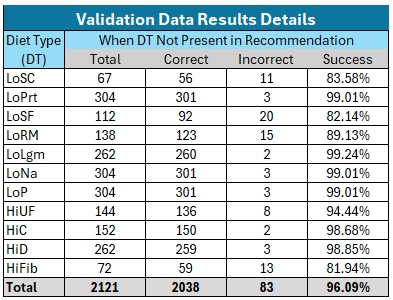
\includegraphics[width=\linewidth]{Figures/vdrdn.png}
    \caption{Results of the validation data when diet type was not present in recommendation.}
\end{table}

These values for accuracy also showed that the model tends to predict better when the diet type is recommended as opposed to when it isn't. A possible reason for this could be that fewer than needed training data was available for better prediction results.

\begin{table}[H]
    \centering
    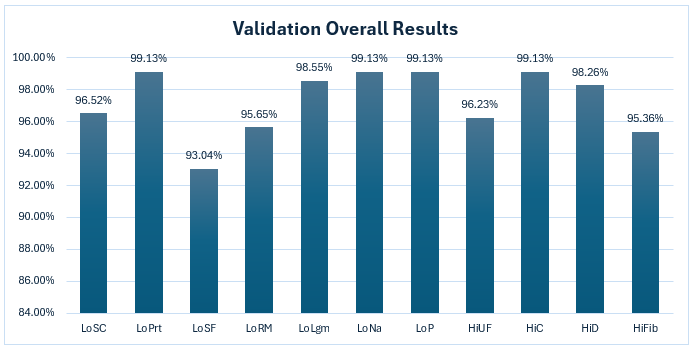
\includegraphics[width=\linewidth]{Figures/barv.png}
    \caption{Results of the overall validation data showing percentage accuracies for each diet type.}
\end{table}

\subsection{Testing Results}
Similarly, for the case of testing data, the overall accuracy of the results among a total of 3806 instances of the food groups combined with the testing data was 96.58\% as shown in \textbf{Table VI}. Success rate shows to vary from 91.04\% to 99.71\% within various diet type recommendations.


\begin{table}[H]
    \centering
    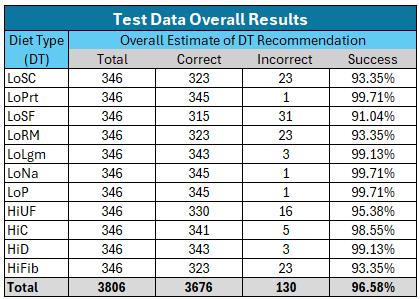
\includegraphics[width=\linewidth]{Figures/tdor.png}
    \caption{Results of the overall testing data.}
\end{table}

\textbf{Table VII} shows the total number of instances where a diet type (DT) was recommended, along with the number of correct and incorrect predictions. Among the 1,719 recommendations, the model correctly identified 1,687 instances, achieving an overall promising accuracy of 98.14\%.

\begin{table}[H]
    \centering
    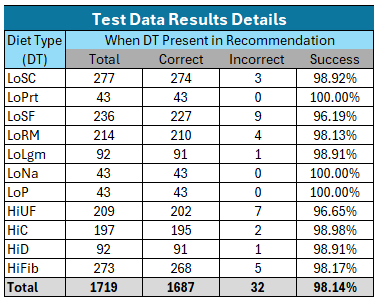
\includegraphics[width=\linewidth]{Figures/tdrdp.png}
    \caption{Results of the testing data when diet type was present in recommendation.}
\end{table}

Finally, \textbf{Table VIII} shows the total number of instances where a diet type (DT) was not recommended and among the 2087 recommendations, the model correctly identified 2038 instances, achieving an overall accuracy of 95.30\%, again reflecting the model's more accuracy in prediction when diet type is recommended as opposed to when it's not. Similar to the validation data, LoSC, LoSF, LoRM and HiFib have contributed to most of these false positives, meaning that these diet types got recommended to some patients by our neural network when they were actually not.


\begin{table}[H]
    \centering
    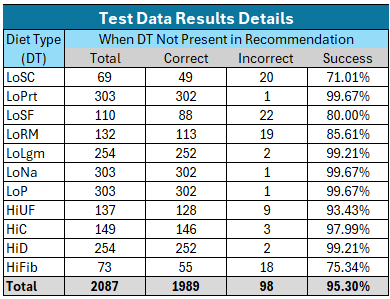
\includegraphics[width=\linewidth]{Figures/tdrdn.png}
    \caption{Results of the testing data when diet type was not present in recommendation.}
\end{table}

\subsection{Confusion Matrices}
A confusion matrix for the validation results show in \textbf{Fig. 6} was also made indicating that the model has a high accuracy of 97.2\%, correctly predicting 1,654 instances where a diet type was recommended (true positives) and 2,038 instances where a diet type was not recommended (true negatives). There were 83 false positives and 20 false negatives, resulting in a precision of 95.2\% and a recall of 98.8\%.

\begin{figure}[H]
    \centering
    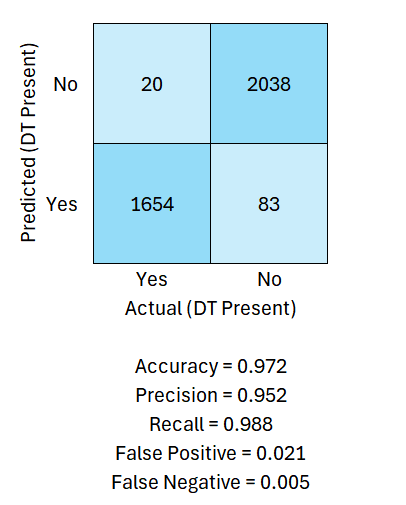
\includegraphics[width=\linewidth]{Figures/confusion_v.png}
    \caption{Confusion matrix compiling the overall validation results.}
\end{figure}

For the testing results, the confusion matrix show in \textbf{Fig. 7} shows an accuracy of 96.5\%, with 1,687 true positives and 1,989 true negatives. There were 98 false positives and 32 false negatives, resulting in a precision of 94.5\% and a recall of 98.1\%. The false positive rate was 2.5\%, and the false negative rate was 0.8\%.

These metrics indicate that the model performs consistently well on both validation and testing datasets, demonstrating high accuracy, precision, and recall in making dietary recommendations.


\begin{figure}[H]
    \centering
    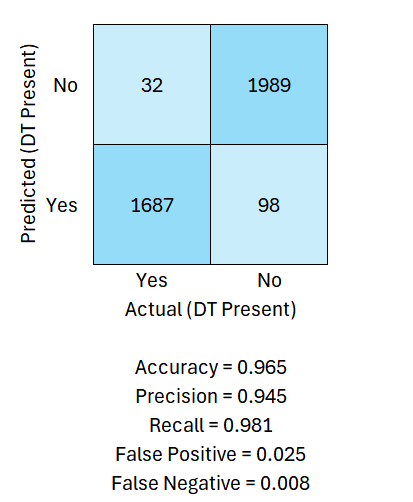
\includegraphics[width=\linewidth]{Figures/confusion_t.png}
    \caption{Confusion matrix compiling the overall testing results.}
\end{figure} 

\subsection{Neural Network Performance}
In conclusion, our neural network model performance was a success exhibiting well over 90\% accuracy. The network has behaved consistently when comparing the result of the testing and validating data as compared by \textbf{Table V} and \textbf{Table IX} and the confusion matrices.

\begin{table}[H]
    \centering
    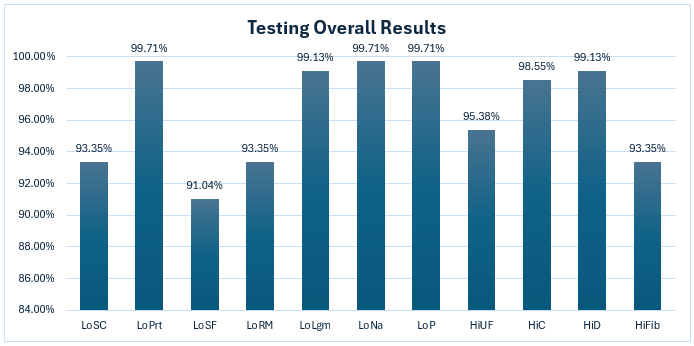
\includegraphics[width=\linewidth]{Figures/bart.png}
    \caption{Results of the overall testing data showing percentage accuracies for each diet type.}
\end{table} 



